\documentclass{article}
\usepackage[margin=0.8in]{geometry}
\usepackage{graphicx}
\usepackage{amsmath, amssymb, hyperref, bm}

\setlength{\parindent}{0pt}
\setlength{\parskip}{0.5em}

\title{Control System Analysis\\of the \textit{Triangle}}
\author{\texttt{dc\&e}}
\date{May 1, 2025\footnote{Last compiled: \today\hfill\texttt{id: 24003}}}
\begin{document}

\maketitle

\tableofcontents


\newpage

\section*{Preface}

This work was carried out by \texttt{dc\&e}, with contributions from:

\begin{enumerate}
  \item Himanshu Paudel
\end{enumerate}

\newpage

\section{Introduction}

We present the mathematical modeling, control system design, and theoretical analysis of the \textit{Triangle} balance robot.

\section{Differential equations the \textit{Triangle}}

In this section, we develop the mathematical model of the \textit{Triangle}, i.e., derive its differential equations. These equations form the basis for stability analysis, control design, and simulation of the control system.

\begin{figure}[ht]
  \centering
  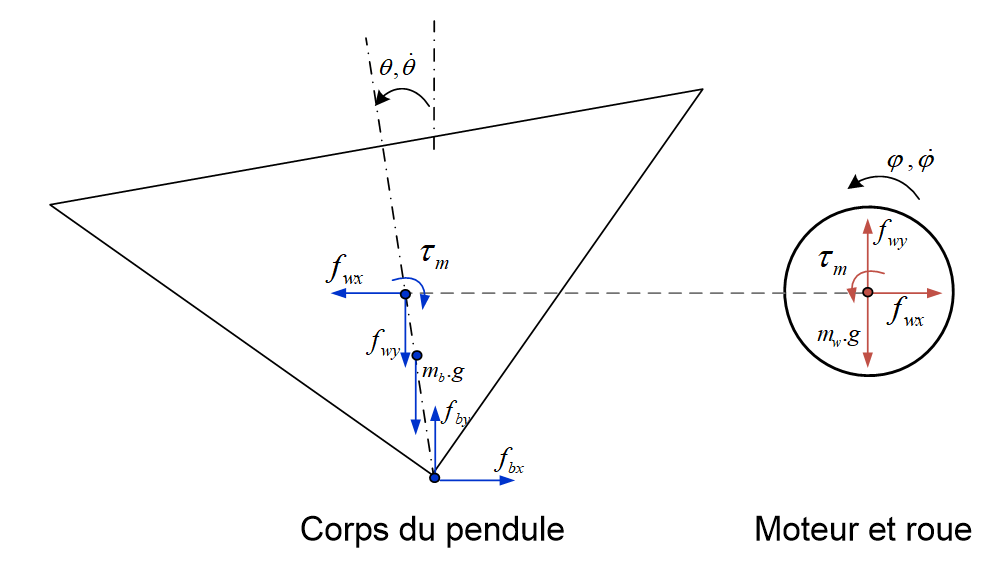
\includegraphics[scale=0.4]{triangle.png}
  \caption{Forces and torques acting on the \textit{Triangle} Balance. Figure inspired from \cite{ipendulum}}
  \label{fig_triangle}
\end{figure}

Fig.(\ref{fig_triangle}) shows the free-body diagram of the \textit{Triangle} where the parameters are defined as following:

\begin{align*}
  \theta &= \text{Pendulum angle} \\
  \varphi &= \text{Wheel angle relative to pendulum} \\
  m_b, I_b, l_b &= \text{Mass, inertia, and center of mass height of pendulum body} \\
  m_w, I_w, l_w &= \text{Mass, inertia, and center of mass height of wheel} \\
  \tau_m &= \text{Motor torque} \\
  \tau_f &= \text{Friction torque} \\
  M &= m_b l_b + m_w l_w \\
  I &= I_b + m_b l_b^2 + m_w l_w^2
\end{align*}

\subsection{Construction of the Lagrangian}

Euler-Lagrange equation is used to derive the differential equation, threfore, we start by expressing the Kinetic energy $T$ and potential energy $V$ of the \textit{Triangle} to compute the Lagrangian as
\begin{equation}
  \label{eqn_lagrangian}
  L=T-V
\end{equation}

The kinetic energy of the \textit{Triangle} is the sum of kinetic energy of the body $T_{b}$, and that of the wheel $T_{w}$. The term $T_{b}$ can be expressed at the sum of the kinetic energy due to the angular motion and the translational motion of the body's center of mass i.e.
\begin{equation}
  T_b=\dfrac{1}{2}\left(I_{b} + m_{b} l_{b}^{2}\right)\dot{\theta}^{2}
\end{equation}

where, $l_{b}\dot{\theta}$ is the linear velocity of the center of mass.\footnote{If a rigid body rotates around a fixed point with angular velocity $\dot{\theta}$, any point on the body located at a distance $r$ from the pivot traces a circular path. The linear velocity $v$ of that point is related to the angular velocity as $v=r\dot{\theta}$.}

The reaction wheel, on the other hand, has three sources of its kinetic energy: (1) rotation about its own axis, (2) rotation of the body about its axis, and (3) translational motion in the inertial frame, resulting from the body's rotation. Therefore, the kinetic energy of the wheel is the sum of its rotational and the translational kinetic energies i.e.

\begin{equation}
  T_w=\dfrac{1}{2}\left(I_{w}(\dot{\theta}+\dot{\varphi})^{2}+m_{w}l_{w}^{2}\dot{\theta}^2\right).
\end{equation}

The total kinetic energy of the \textit{Triangle} can be expressed as
\begin{equation}
  \begin{split}
    T&=T_{b}+T_{w}\\
    &=\dfrac{1}{2}\left(I_{b} + m_{b} l_{b}^{2}\right)\dot{\theta}^{2}+\dfrac{1}{2}\left(I_{w}(\dot{\theta}+\dot{\varphi})^{2}+m_{w}l_{w}^{2}\dot{\theta}^2\right)\\
    &= \frac{1}{2}\left(\left(I_b+m_{b}l_{b}^{2}+I_{w}+m_{w}l_{w}^{2}\right)\dot{\theta}^2+2I_{w}\dot{\theta}\dot{\varphi}+I_{w}\dot{\varphi}^2\right)\\
    &= \frac{1}{2}\left(I\dot{\theta}^2+I_{w}\dot{\theta}^{2}+2I_{w}\dot{\theta}\dot{\varphi}+I_{w}\dot{\varphi}^2\right)\\
    &= \frac{1}{2}\left(I\dot{\theta}^{2}+I_{w}(\dot{\theta}+\dot{\varphi})^{2}\right)
  \end{split}
\end{equation}

where, $I=I_b+m_{b}l_{b}^{2}+m_{w}l_{w}^{2}$.

We know that a mass' potential energy depends on its vertical position (the good old $-mgh$). Both the body and the wheel rotates with the same angle $\theta$ with respect to the vertical. Therefore, as the body rotates, both center of mass move in a circular arc of radius $l_{b}$ and $l_{w}$ respectively. The vertical height of each center of mass relative to the pivot is:
\begin{equation*}
  \begin{split}
    h_{b}&=-l_{b}\cos\theta\\
    h_{w}&=-l_{w}\cos\theta
  \end{split}
\end{equation*}

where the terms are negative because $\theta=0$. The total potential energy of the \textit{Triangle} is the sum of potential energies of the body and the wheel, i.e.
\begin{equation}
  \begin{split}
    V&=-m_{b}gh_{b}-m_{w}gh_{w}\\
    &=-(m_{b}gl_{b}+m_{w}gl_{w})\cos\theta\\
    &=-Mg\cos\theta
  \end{split}
\end{equation}

where, $M=m_{b}l_{b}+m_{w}l_{w}$.

We can now use Eqn.(\ref{eqn_lagrangian}) to compute the Lagrangian.

\begin{equation}
  L=T-V=\frac{1}{2}I\dot{\theta}^{2}+\dfrac{1}{2}I_{w}(\dot{\theta}+\dot{\varphi})^{2}+Mg\cos\theta
\end{equation}

\subsection{Equations of motion}

\subsubsection*{Equation of motion of the body}

The Euler-Lagrange equation for the body is expressed as
\begin{equation}
  \label{eqn_elb}
  \dfrac{d}{dt}\left( \dfrac{\partial L}{\partial\dot{\theta}} \right)-\dfrac{\partial L}{\partial\theta}=\tau_{f}-\tau_{m}.
\end{equation}

Computing the terms involved.
\begin{equation}
  \begin{split}
    \dfrac{\partial L}{\partial\dot{\theta}}&=I\dot{\theta}+I_{w}(\dot{\theta}+\dot{\varphi})
    \implies\dfrac{d}{dt}\left(\dfrac{\partial L}{\partial\dot{\theta}}\right)=(I+I_{w})\ddot{\theta}+I_{w}\ddot{\varphi}\\
    \dfrac{\partial L}{\partial\theta}&=-Mg\sin\theta
    \end{split}
\end{equation}

Plugging in the terms to Eqn.(\ref{eqn_elb}), we get the equation of motion of the body.

\begin{equation}
  \label{eqn_tempb}
  (I+I_{w})\ddot{\theta}+I_{w}\ddot{\varphi}+Mg\sin\theta=\tau_{f}-\tau_{m}
\end{equation}

\subsubsection*{Equation of motion of the wheel}

The Euler-Lagrange equation for the wheel is expressed as
\begin{equation}
  \label{eqn_elw}
  \dfrac{d}{dt}\left(\dfrac{\partial L}{\partial\dot{\varphi}} \right)-\dfrac{\partial L}{\partial\varphi}=\tau_{f}-\tau_{m}.
\end{equation}

Similar to what we did for the body, computing the terms involved,

\begin{equation}
  \begin{split}
  \dfrac{\partial L}{\partial \dot{\varphi}}&=I_w (\dot{\theta} + \dot{\varphi})\implies\dfrac{d}{dt}\left(\dfrac{\partial L}{\partial\dot{\varphi}} \right)=I_{w}(\ddot{\theta}+\ddot{\varphi})\\
  \dfrac{\partial L}{\partial\varphi}&=0
  \end{split}
\end{equation}

Plugging the expression into the Eqn.(\ref{eqn_elw}), we get

\begin{equation}
  \label{eqn_tempw}
  \begin{split}
    I_{w}(\ddot{\theta}+\ddot{\varphi})&=\tau_{m}-\tau_{f}\\
    \implies\ddot{\varphi}&= \dfrac{\tau_m - \tau_f}{I_w} - \ddot{\theta}\\
  \end{split}
\end{equation}

\subsubsection*{Equations of motion of the system}

We can observe that equation of motion of both body and the wheel are coupled with double derivatives as both Eqn.(\ref{eqn_tempb}) and  Eqn.(\ref{eqn_tempw}) contains both terms $\ddot{\theta}$ and $\ddot{\varphi}$. Now we will derive separate equation of motion for each of them by decoupling the double derivative terms.

We begin by plugging Eqn.(\ref{eqn_tempw}) into Eqn.(\ref{eqn_tempb}).

\begin{equation}
  \begin{split}
    \label{eqn_eomb}
    (I+I_{w})\ddot{\theta}+I_{w}\left(\dfrac{\tau_{m}-\tau_{f}}{I_{w}}-\ddot{\theta}\right)+Mg\sin\theta&=\tau_{f}-\tau_{m}\\
  I\ddot{\theta}=Mg\sin\theta-\tau_{m}+\tau_{f}\\
  \implies\ddot{\theta}=\dfrac{Mg\sin\theta-\tau_{m}+\tau_{f}}{I}
  \end{split}
\end{equation}

Plugging the expression in Eqn.(\ref{eqn_tempw}) gives us

\begin{equation}
  \label{eqn_eomw}
  \ddot{\varphi} = \dfrac{(I + I_w)(\tau_m - \tau_f)}{I I_w} - \dfrac{M g \sin\theta}{I}
\end{equation}

Eqn.(\ref{eqn_eomb}) and Eqn.(\ref{eqn_eomw}) are the equations of motion of the \textit{Triangle}.

\subsection{First order form}
\begin{center}
  TODO
\end{center}

\section{Stability analysis and controller design}

The goal of this section is to design control law for the \textit{Triangle} by using the mathematical tools of the control theory by trying our best to prove our assumptions so that we are comfortable with what we believe.

The goal of the controller is to regulate $\theta$,  $\dot{\theta}$, and $\dot{\varphi}$ to zero. We're not concerned with $\varphi$ at the moment—that's something for a future project. We will begin by performing mathematical analysis proving why we cannot have smooth single control law which can swing up and balance the \textit{Triangle}. That being done, we are naturally lead to implementing two controllers, one for the swing-up and the next for stabilization. Each of them are discussed in detail. Finally, the question of when to switch from swing-up to stabilization is addressed.

\subsection{A global asymptotic controller}

In this section we apply Brockett's condition to check if a single global asymptotic controller can do the job of balancing the \textit{Triangle} from any initial condition.
\begin{center}
  TODO
\end{center}

\subsection{Stabilizer}

\subsubsection*{Lyapunov function}

Since we are interested only on $\theta$,  $\dot{\theta}$, and $\dot{\varphi}$, we design an energy like Lyapunov function

\begin{equation}
  V = \frac{1}{2} I \dot{\theta}^2 + MgL (1 - \cos\theta) + \frac{1}{2} k_1 \dot{\varphi}^2, \quad k_1 > 0
\end{equation}

where the first two terms represents the mechanical energy of robot body. We synthesize the third, wheel damping, term as we are interested in the angular rate of the wheel as well. The term $k_{1}$ represents the magnitude of damping. It should be noted that we do not require custom gains on other terms ($I$, $M$, $g$, and $L$) because they are provided by physics and system parameters.

Following the steps of Lyapunov analysis, now we compute the time derivative $V$, and plug in the expressions from the equations of motion Eqn.(\ref{eqn_eomb}) and Eqn.(\ref{eqn_eomw}).

\begin{align}
  \dot{V} &= I \dot{\theta} \ddot{\theta} + MgL \dot{\theta} \sin\theta + k_1 \dot{\varphi} \ddot{\varphi} \nonumber \\
          &= \dot{\theta}(2MgL \sin\theta - \tau_m) + k_1 \dot{\varphi}\left(\frac{(I + I_w)}{I I_w}\tau_m - \frac{MgL \sin\theta}{I}\right)
  \label{eqn_vdot}
\end{align}

We now, \textit{search for} the control law forces $\dot{V}$ to be negative semi-definite i.e. $\dot{V}\leq0$.

\begin{equation}
  \tau_m = 2MgL \sin\theta + k_2 \dot{\theta} - \tau_{f}- k_1 \frac{(I + I_w)}{I I_w} \dot{\varphi}
  \label{eqn_ctrl}
\end{equation}

Plugging in the expression of control torque into Eqn.{\ref{eqn_vdot}} to make sure if is $\dot{V}$ indeed negative semi-definite.

\begin{equation}
  \dot{V} = -k_2 \dot{\theta}^2 - k_1 \frac{(I + I_w)^2}{I^2 I_w^2} \dot{\varphi}^2 \leq 0
\end{equation}

When $\dot{V}$ is negative semi-definite, we ask LaSalle for help!

\subsubsection*{LaSalle's invariance principle}

LaSalle's principle requires finding the largest invariant set where $\dot{V} = 0$:

\begin{enumerate}
  \item From \eqref{eqn_vdot}, $\dot{V} = 0$ implies $\dot{\theta} = 0$ and $\dot{\varphi} = 0$

  \item Substituting $\dot{\theta} = \dot{\varphi} = 0$ into \eqref{eqn_eomb} and \eqref{eqn_eomw}:
  \begin{align}
    0 &= MgL\sin\theta - \tau_m \label{eq:theta_eq} \\
    0 &= \frac{(I + I_w)\tau_m}{I I_w} - \frac{MgL\sin\theta}{I} \label{eq:phi_eq}
  \end{align}

  \item Substituting the control law \eqref{eqn_ctrl} with $\dot{\theta} = \dot{\varphi} = 0$:
  \begin{equation}
    \tau_m = 2MgL\sin\theta
  \end{equation}

  \item Combining with \eqref{eq:theta_eq}:
  \begin{equation}
      MgL\sin\theta = 2MgL\sin\theta \implies \sin\theta = 0
  \end{equation}
\end{enumerate}

The only invariant solutions are:
\begin{enumerate}
  \item$\theta=0,\dot{\theta}=0,\dot{\varphi}=0$ (desired upright equilibrium)
  \item$\theta=\pi,\dot{\theta}=0,\dot{\varphi}=0$ (unstable downward position)
\end{enumerate}

Since $V$ is radially unbounded and the downward position is unstable, all trajectories converge to the upright equilibrium $(\theta, \dot{\theta}, \dot{\varphi}) = (0, 0, 0)$.

\subsubsection*{The stabilizer control law}

Our controller, in nonlinear form, as expressed in Eqn.(\ref{eqn_ctrl}) is
\begin{equation*}
  \tau_m=2MgL\sin\theta+k_{2}\dot{\theta}-\tau_{f}-k_1\frac{(I+I_w)}{II_w}\dot{\varphi}
\end{equation*}

The first term compensates gravity, second damps the robot velocity, third compensates friction, and the last damps the wheel velocity. If we are near the equilibrium angle, then gravity compensation can be considered linear with the approximation $\sin\theta\approx\theta$ which linearizes the control law to be
\begin{equation}
  \tau_m=k_{p}\theta+k_d\dot{\theta}+k_{w}\dot{\varphi}-\tau_{f}.
\end{equation}

This requires us to determine the friction of the motor. However, the classic action of neglecting friction leads to simpler linear control law
\begin{equation}
  \tau_m=k_{p}\theta+k_d\dot{\theta}+k_{w}\dot{\varphi}
\end{equation}

where, $k_{p}=2MgL$, $k_{d}=k_{2}$, and $k_{w}=-k_{1}(I+I_w)/(II_{w})$.

\subsection{Swing-up controller}

The goal of the swing-up controller is to “wake up” the \textit{Triangle} from its stable equilibrium and bring it closer to the upright position, enabling the stabilizer to take over and perform the actual balancing. In this section, we discuss and design the swing-up controller, beginning with physical intuition and mathematical analysis to identify key parameters.

Our study of swing-up controllers naturally began with studying the swing-up of the classic inverted pendulum or the Furuta pendulum. Therefore, we will start our analysis with the swing-up for those pendulums and make some inferences about what the swing-up for the \textit{Triangle} looks like—or rather, does not look like.

\subsubsection*{Swing-up for inverted pendulum and Furuta pendulum}

Figs.~\ref{fig_swing}A and B show schematic diagrams of the Furuta pendulum and the cart-pole inverted pendulum system. The Furuta pendulum consists of a motorized rotating base to which a passive pendulum is attached via a bearing. The pendulum is unactuated and responds to the angular motion of the base. Swing-up is achieved by oscillating the base back and forth, thereby injecting energy into the pendulum until it enters the vicinity of the upright position, where a stabilizing controller can take over.

Similarly, Figs.~\ref{fig_swing}C and D depict the cart-pole system, where linear translation of a cart on a belt emulates base rotation. As with the Furuta pendulum, the swing-up phase consists of back-and-forth motion of the cart to accumulate energy in the pendulum.

\begin{figure}[ht]
  \centering
  \raisebox{-.5\height}{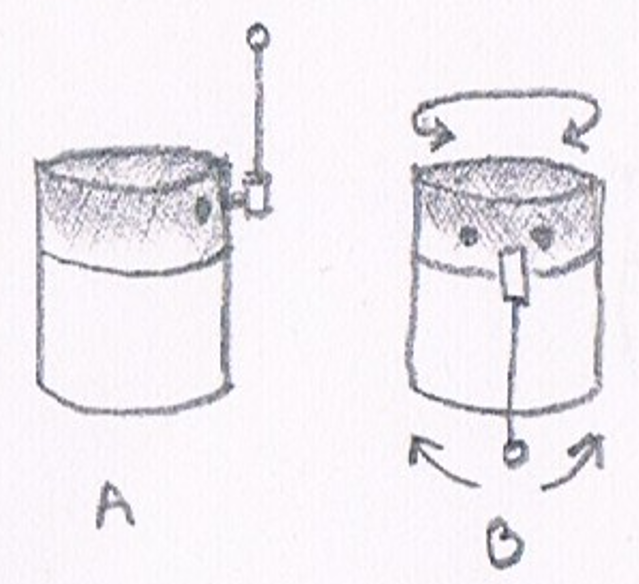
\includegraphics[scale=0.2]{furuta.png}}\hspace{1cm}
  \raisebox{-.5\height}{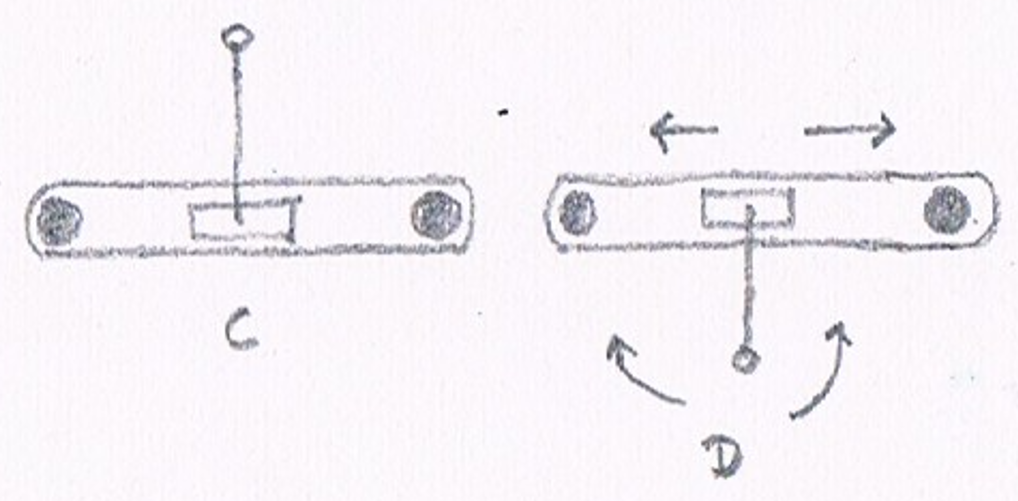
\includegraphics[scale=0.2]{invpen.png}}
  \caption{
    \centering
    \parbox{0.8\linewidth}{
      A: Balanced Furuta pendulum. B: Swing-up of Furuta pendulum.\\
      C: Balanced inverted pendulum. D: Swing-up of inverted pendulum.
    }
  }
  \label{fig_swing}
\end{figure}

In both classical cases, two crucial properties enable successful swing-up:

\begin{enumerate}
  \item The pendulum's motion is directly influenced by external torques applied to the base. The energy required for swing-up is externally supplied.
  \item The pendulum is free to swing around the stable equilibrium (hanging down), allowing multiple passes through the bottom position to gradually increase its energy.
\end{enumerate}

In contrast, the \textit{Triangle} is based on a fundamentally different actuation and configuration setup:

\begin{itemize}
  \item \textbf{Momentum-based actuation:} It relies on internal actuation via a reaction wheel. This means that the pendulum's motion results from internal momentum exchange, not direct torque on a pivoted base.

  \item \textbf{Restricted motion domain:} Due to the geometry of the triangle-shaped body, the system cannot rotate freely around the stable equilibrium point. The body rests flat on the ground and cannot swing through the downward position repeatedly. As a result, traditional energy-pumping swing-up strategies—which rely on oscillating the pendulum around its lowest point—are not applicable.

  \item \textbf{No natural oscillating cycle:} Once the \textit{Triangle} body falls to the ground, there is no passive return to a previous state without deliberate re-actuation. This lack of reversible dynamics further invalidates classical swing-up methods.
\end{itemize}

\subsubsection*{Swing-up for the \textit{Triangle}}

Based on the intuition developed above, it is clear that a fundamentally different approach is required for swing-up control in the \textit{Triangle}. Unlike conventional systems that exploit natural dynamics and repeated oscillations, the controller must instead perform a deliberate, one-shot energy transfer from the reaction wheel to the body. One possible method is to plan a trajectory from the resting position to the upright configuration and follow it using a precomputed, learned, or real-time trajectory optimization. While this approach can yield smooth motion, it is highly sensitive to model accuracy and initial conditions, and it demands significant design and implementation effort—an approach we will not pursue here but instead reserve as a potential direction for future work should anyone be interested.

Instead, we adopt a simpler strategy: an impulse-like, open-loop energy injection. This method involves rapidly spinning the reaction wheel and then braking or reversing it to ``kick'' the \textit{Triangle} upright. It is computationally light, straightforward to implement, and well-suited for our system.

The impulse-like, single-shot swing-up strategy consists of three main stages, each with tunable parameters. First, the reaction wheel is spun up by applying a constant angular velocity for a fixed duration, allowing it to accumulate angular momentum. This spin-up phase can involve either a gradual acceleration or direct velocity set-point control. To mitigate overshoot, the target angular velocity can be made a function of the initial rest angle of the \textit{Triangle}. Next, a sudden deceleration of the wheel transfers the accumulated momentum to the body. This is typically achieved via braking or reversing the wheel's direction. The aggressiveness of this deceleration—whether abrupt or gradual—affects the strength and smoothness of the resulting lift. Finally, if the momentum transfer is effective, the body swings upward toward the upright position, where the stabilizer can be activated to take control.

\subsubsection{Determination of the wheel's speed for swing-up}

In this section, we determine the minimum initial angular rate that the reaction wheel must achieve before braking to safely approach the unstable equilibrium. The optimal angular rate for the reaction wheel during swing-up must balance energy injection, system dynamics, and overshoot avoidance. We utilize two fundamental physical principles governing the \textit{Triangle}: conservation of energy and momentum exchange. Throughout this analysis, we neglect motor friction and assume instantaneous deceleration\footnote{I am very eager to generalize this analysis for non-zero motor friction and finite deceleration time after first validating these simplified results in simulation with Himanshu. -rms}.

\subsubsection*{Conservation of Energy}

The kinetic energy of the rotating reaction wheel drives the change in potential energy of the \textit{Triangle} body during swing-up.

Assume the \textit{Triangle} starts at rest with initial angle $\theta_{0}$. To pump energy into the system via the reaction wheel's kinetic energy such that the angle approaches zero, the required potential energy change is:
\begin{equation*}
  \Delta U = Mg(-\cos\theta_{0}+\cos0) \leq \frac{1}{2}I_{w}\dot{\varphi}^{2}
\end{equation*}

Let $\dot{\varphi}_{0}$ be the minimum initial angular velocity of the reaction wheel needed to achieve this energy transfer after braking:
\begin{equation*}
  \begin{split}
    \Delta U &= \frac{1}{2}I_{w}\dot{\varphi}_{0}^{2} = Mg(1-\cos\theta_{0})\\
    \implies \dot\varphi_{0} &= \sqrt{\frac{2MgL(1-\cos\theta_{0})}{I_{w}}}
  \end{split}
\end{equation*}

This expression provides a baseline lower bound for the initial angular velocity of the reaction wheel. However, it doesn't account for the dynamics of how energy transfers from the wheel to the \textit{Triangle} body, particularly during momentum exchange.

\subsubsection*{Momentum Transfer Dynamics}

The angular momentum conservation for the \textit{Triangle} system is:
\begin{equation*}
  (I_{b} + I_{w})\dot{\theta} + I_{w}\dot{\varphi} = 0
\end{equation*}

When the wheel brakes suddenly, its momentum transfers to the body, producing an angular velocity:
\begin{equation*}
  \dot{\theta} = -\frac{I_{w}}{I_{b} + I_{w}}\dot{\varphi}
\end{equation*}

As the body's kinetic energy converts to potential energy during the rise, the peak angle $\theta_{p}$ satisfies:
\begin{equation*}
  \begin{split}
    \frac{1}{2}(I_{b} + I_{w})\dot{\theta}^{2} &= Mg(1 - \cos\theta_{p})\\
    \frac{I_{w}^{2}\dot{\varphi}^{2}}{2(I_{b} + I_{w})} &= Mg(1 - \cos\theta_{p})\\
    \theta_{p} &= \cos^{-1}\left(1 - \frac{I_{w}^{2}\dot{\varphi}^{2}}{2(I_{b} + I_{w})Mg}\right)
  \end{split}
\end{equation*}

For small angles ($\theta_{p} \approx 0^{\circ}$), using the Taylor series approximation $1 - \cos\theta \approx \theta^{2}/2$:
\begin{equation*}
\theta_{p} \approx \sqrt{\frac{I_{w}^{2}\dot{\varphi}_{0}^{2}}{(I_{b} + I_{w})Mg}}
\end{equation*}

This analysis captures the transient swing-up behavior and predicts the body's state after wheel braking, which depends on the system parameters (masses and inertias).

\subsubsection*{Implementation Procedure}

The energy conservation approach gives us a fundamental lower bound on the required wheel speed for swing-up, but it's inherently a static analysis—it tells us whether there's enough energy in the system, but not how that energy actually moves or is transferred. On the other hand, using momentum transfer through the system's differential equations of motion makes the dynamic interaction between the wheel and the body much more explicit. This setup naturally includes motor dynamics as well: the motor torque $\tau_m(t)$ shows up directly in the angular momentum equations, the electrical behavior is described by $L\dot{i} + Ri = V - k_e\dot{\varphi}$, and the link between torque and current is given by $\tau_m = k_t i$. Time-varying inputs like braking profiles can also be handled through $\dot{\varphi}(t)$. So while energy analysis gives us a simple scalar condition, the momentum-based approach adds temporal resolution, which is key for modeling motor behavior, accounting for power electronics limits, and designing realistic braking strategies—all of which are important for real-world simulation and implementation.

Having performed the analysis following are the proposed implementation procedure, practicability of which is yet to be verified.

\begin{enumerate}
  \item Calculate $\dot{\varphi}_{0}$ from energy conservation
  \item Verify if momentum transfer produces sufficient $\theta_{p}$ for this $\dot{\varphi}_{0}$
  \item If necessary, increase $\dot{\varphi}$ until both conditions are satisfied
  \item Validate the process and the parameter through experimental testing
\end{enumerate}

\subsubsection{Determination of switching thresholds}

Using a time-based threshold to switch from swing-up to stabilization is unsuitable because the system's motion depends on the \textit{Triangle}'s initial orientation. The switching must occur late enough that the body approaches upright with sufficient momentum but, at the same time, early enough for the stabilizer to act before the body falls away.

That being said, we have three possible parameters to use as thresholds for switching from swing-up to stabilization: $\theta$ (body angle), $\dot{\theta}$ (body angular velocity), and $\dot{\varphi}$ (wheel speed). Among these, $\theta$ and $\dot{\theta}$ directly characterize the body's orientation and motion, making them the primary indicators for whether the system is near the upright position and slow enough for the stabilizer to engage effectively. The wheel speed $\dot{\varphi}$, while available, is optional---after all, during the momentum exchange process used in swing-up, the wheel is typically decelerated or even brought close to rest. By the time the body is upright, the energy transfer is largely complete, and the wheel's velocity provides little additional information about the body's readiness for stabilization. Therefore, relying on $\theta$ and $\dot{\theta}$ is both sufficient and more directly relevant to the switching decision. We are left with an important question:
\begin{quote}
  \textit{What should be the values of the thresholds for angle $\theta_{\text{th}}$ and angular velocity $\dot{\theta}_{\text{th}}$?}
\end{quote}

We attempt to analytically estimate the switching thresholds $\theta_{\text{th}}$ and $\dot{\theta}_{\text{th}}$ by examining the region of attraction of the stabilizing controller around the upright position. The key idea is to ensure that, once the swing-up phase ends, the system's state lies within a neighborhood where the stabilizer can drive the state to equilibrium reliably.

Assuming a linear stabilizer, the linearized dynamics around $\theta = 0$ can be used to compute the region in which the controller guarantees convergence. The linearized system is obtained by expanding the nonlinear equations around $\theta = 0$ and $\dot{\theta} = 0$:

\begin{equation*}
\ddot{\theta} \approx \frac{Mg\theta - \tau_m + \tau_f}{I}
\end{equation*}

This yields a linear approximation:
\begin{equation*}
\ddot{\theta} = \frac{Mg}{I}\theta + \text{control terms}
\end{equation*}

The region of attraction of such a linear system can be bounded using a Lyapunov function or by simulating trajectories from various initial conditions and checking for convergence. In practice, a reasonable conservative estimate is to select $\theta_{\text{th}}$ such that $|\theta| < \theta_{\text{max}}$ and $|\dot{\theta}| < \dot{\theta}_{\text{max}}$, where $\theta_{\text{max}}$ and $\dot{\theta}_{\text{max}}$ are chosen so that the linear controller performs well within this domain.

These values will be determined by analyzing the eigenvalues of the linearized system matrix to determine bounds for stability and validated using simulations (i.e. sweep through $(\theta, \dot{\theta})$ values and check convergence). This approach provides a more design-based method for selecting switching thresholds rather than relying purely on trial and error.

\bibliographystyle{plain}
\bibliography{references}

\end{document}
